El entorno gráfico cuenta con 13 botones en total, 12 para mover el brazo en los ejes x,y,z; y uno para accionar la pinza.
\par
En el código se inicializa el id del producto y el del proveedor del arduino uno. Se procede a reconocer los puertos disponibles y comparar el identificador del producto y el del proveedor conectados con los previamente seteados. Si coinciden, en la variable arduino uno port name se copia la información referente al puerto de serie, que se utilizará luego para inicializar el nombre del puerto. 
\par
Se procede a verificar que, dentro de la comunicación serial, el baudrate, los bits, la paridad, etc. sean los requeridos para seguir con el proceso. Se espera por un dato de entrada, dicha información se lee y se depura. En caso de no poder hacerlo se imprime un error. 
\par
Al presionar un botón, ejemplo -x se verifica que se pueda escribir el puerto de serie y, si es así, se envía un valor, en este caso, de -100.
\begin{figure}[!htb]
  \begin{center}
    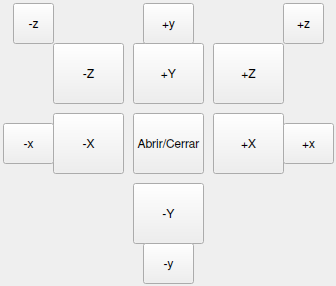
\includegraphics[width=0.5\textwidth]{imagenes/GUIscreenShot.png}
  \end{center}
  \caption{Implementación interfaz gráfica}
  \label{fig:GUI}
\end{figure}
\FloatBarrier

